\documentclass{beamer}
\input{../utils/preamble}
\createdgmtitle{9}
%--------------------------------------------------------------------------------
\begin{document}
%--------------------------------------------------------------------------------
\begin{frame}[noframenumbering,plain]
\titlepage
    \resetonslide
\end{frame}
%=======
\begin{frame}{Recap of Previous Lecture}
	\myfootnotewithlink{https://arxiv.org/abs/2006.11239}{Ho J. Denoising Diffusion Probabilistic Models, 2020}
	\begin{block}{ELBO of the Gaussian Diffusion Model}
		\vspace{-0.7cm}
		\begin{multline*}
			\cL_{\bphi, \btheta}(\bx) =  {\color{olive}\bbE_{q(\bx_1 | \bx_0)} \log \pt(\bx_0 | \bx_1)} - {\color{violet}\KL\bigl(q(\bx_T | \bx_0) \| p(\bx_T)\bigr)} - \\
			- \sum_{t=2}^\top  \underbrace{ \bbE_{q(\bx_t | \bx_0)}\KL \bigl(q(\bx_{t-1} | \bx_t, \bx_0) \| \pt(\bx_{t-1} | \bx_t)\bigr)}_{\cL_t}
		\end{multline*}
		\vspace{-1.0cm}
	\end{block}
	\begin{align*}
		q(\bx_{t-1} | \bx_t, \bx_0) &= \cN(\tilde{\bmu}_t(\bx_t, \bx_0), \tilde{\beta}_t \bI), \\
		\pt(\bx_{t - 1} | \bx_t) &= \cN \bigl(\bmu_{\btheta, t}(\bx_t), {\color{violet}\bsigma_{\btheta, t}^2(\bx_t)}\bigr)
	\end{align*}
	It is assumed that ${\color{violet}\bsigma_{\btheta, t}^2(\bx_t) = \tilde{\beta}_t \bI}$.
	\[
		\cL_t = \bbE_{q(\bx_t | \bx_0)} \left[\frac{1}{2\tilde{\beta}_t} \bigl\| \tilde{\bmu}_t(\bx_t, \bx_0) - \bmu_{\btheta, t}(\bx_t) \bigr\|^2  \right]
	\]
\end{frame}
%=======
\begin{frame}{Recap of Previous Lecture}
	\myfootnotewithlink{https://arxiv.org/abs/2006.11239}{Ho J. Denoising Diffusion Probabilistic Models, 2020}
	\[
		\cL_t = \bbE_{\color{violet}q(\bx_t | \bx_0)} \left[ {\color{olive}\frac{1}{2\tilde{\beta}_t}} \bigl\| \tilde{\bmu}_t(\bx_t, \bx_0) - \bmu_{\btheta, t}(\bx_t) \bigr\|^2  \right]
	\]
	\vspace{-0.3cm}
	\begin{block}{Reparameterization}
		\vspace{-0.7cm}
		\begin{align*}
			\tilde{\bmu}_t(\bx_t, \bx_0) &= \frac{1}{\sqrt{\alpha_t}} \cdot \bx_t - \frac{1 - \alpha_t}{\sqrt{\alpha_t (1 - \bar{\alpha}_t)}} \cdot \bepsilon \\
			\bmu_{\btheta, t}(\bx_t) &= \frac{1}{\sqrt{\alpha_t}} \cdot \bx_t - \frac{1 - \alpha_t}{\sqrt{\alpha_t (1 - \bar{\alpha}_t)}} \cdot \bepsilon_{\btheta, t}({\color{teal}\bx_t})
		\end{align*}
		\vspace{-0.7cm}
	\end{block}
	\vspace{-0.2cm}
	\[
		\cL_t  =	 \bbE_{\color{violet}\bepsilon \sim \cN(0, \bI)} \left[ \frac{(1 - \alpha_t)^2}{2\tilde{\beta}_t \alpha_t (1 - \bar{\alpha}_t)} \Bigl\| \bepsilon - \bepsilon_{\btheta, t}\bigl( {\color{teal}\sqrt{\bar{\alpha}_t} \bx_0 + \sqrt{1 - \bar{\alpha}_t} \bepsilon}\bigr) \Bigr\|^2 \right]
	\]
	At each step in the reverse diffusion process, our goal is to predict the noise~$\bepsilon$ added by the forward process!
	\begin{block}{Simplified Objective}
		\vspace{-0.7cm}
		\[
			 \cL_{\text{simple}} = \bbE_{t \sim U\{2, T\}} \bbE_{\bepsilon \sim \cN(0, \bI)} \Bigl\| \bepsilon - \bepsilon_{\btheta, t}\bigl( \sqrt{\bar{\alpha}_t} \bx_0 + \sqrt{1 - \bar{\alpha}_t} \bepsilon\bigr) \Bigr\|^2 
		\]
	\end{block}
\end{frame}
%=======
\begin{frame}{Recap of Previous Lecture}
	\myfootnotewithlink{https://arxiv.org/abs/2006.11239}{Ho J. Denoising Diffusion Probabilistic Models, 2020}
	\begin{block}{Training DDPM}
		\begin{enumerate}
			\item Draw a sample $\bx_0 \sim \pd(\bx)$.
			\item Sample a timestep $t \sim U\{1, T\}$ and noise $\bepsilon \sim \cN(0, \bI)$.
			\item Obtain the noisy image: $\bx_t = \sqrt{\bar{\alpha}_t} \cdot \bx_0 + \sqrt{1 - \bar{\alpha}_t} \cdot \bepsilon$.
			\item Compute the loss: $ \cL_{\text{simple}} = \| \bepsilon - \bepsilon_{\btheta, t}(\bx_t) \|^2 $.
		\end{enumerate}
	\end{block}
	\begin{block}{Sampling with DDPM}
		\begin{enumerate}
			\item Sample $\bx_T \sim \cN(0, \bI)$.
			\item Compute the mean of $\pt(\bx_{t-1} | \bx_t) = \cN(\bmu_{\btheta, t}(\bx_t), \sigma_t^2 \cdot \bI)$:
			\[
				\bmu_{\btheta, t}(\bx_t) = \frac{1}{\sqrt{\alpha_t}} \cdot \bx_t - \frac{1 - \alpha_t}{\sqrt{\alpha_t (1 - \bar{\alpha}_t)}} \cdot \bepsilon_{\btheta, t}(\bx_t)
			\]
			\vspace{-0.3cm}
			\item Generate a denoised image: $\bx_{t - 1} = \bmu_{\btheta, t}(\bx_t) +  \sigma_t \cdot \bepsilon$, where $\bepsilon \sim \cN(0, \bI)$.
		\end{enumerate}
	\end{block}
\end{frame}
%=======
\begin{frame}{Outline}
	\tableofcontents
\end{frame}
%=======
\section{Continuous-Time Normalizing Flows}
%=======
\begin{frame}{Discrete-Time Normalizing Flows}
	\myfootnotewithlink{https://lilianweng.github.io/lil-log/2018/10/13/flow-based-deep-generative-models.html}{https://lilianweng.github.io/lil-log/2018/10/13/flow-based-deep-generative-models.html}
	\vspace{-0.3cm}
	\begin{block}{Change of Variable Theorem (CoV)}
		Let $\bx$ be a random variable with density $p(\bx)$, and let $\bff: \bbR^m \rightarrow \bbR^m$ be a differentiable and \textbf{invertible} transformation. If $\bz = \bff(\bx)$, $\bx = \bff^{-1}(\bz) = \bg(\bz)$, then
		\vspace{-0.3cm}
		\[
			p(\bx) = p(\bz) |\det(\bJ_{\bff})| = p(\bz) \left|\det \left( \frac{\partial \bz}{\partial \bx} \right) \right| = p(\bff(\bx)) \left|\det \left(  \frac{\partial \bff(\bx)}{\partial \bx} \right) \right|
		\]
		\vspace{-0.5cm}
	\end{block}
	\eqpause

	\vspace{-0.3cm}
	\begin{figure}
		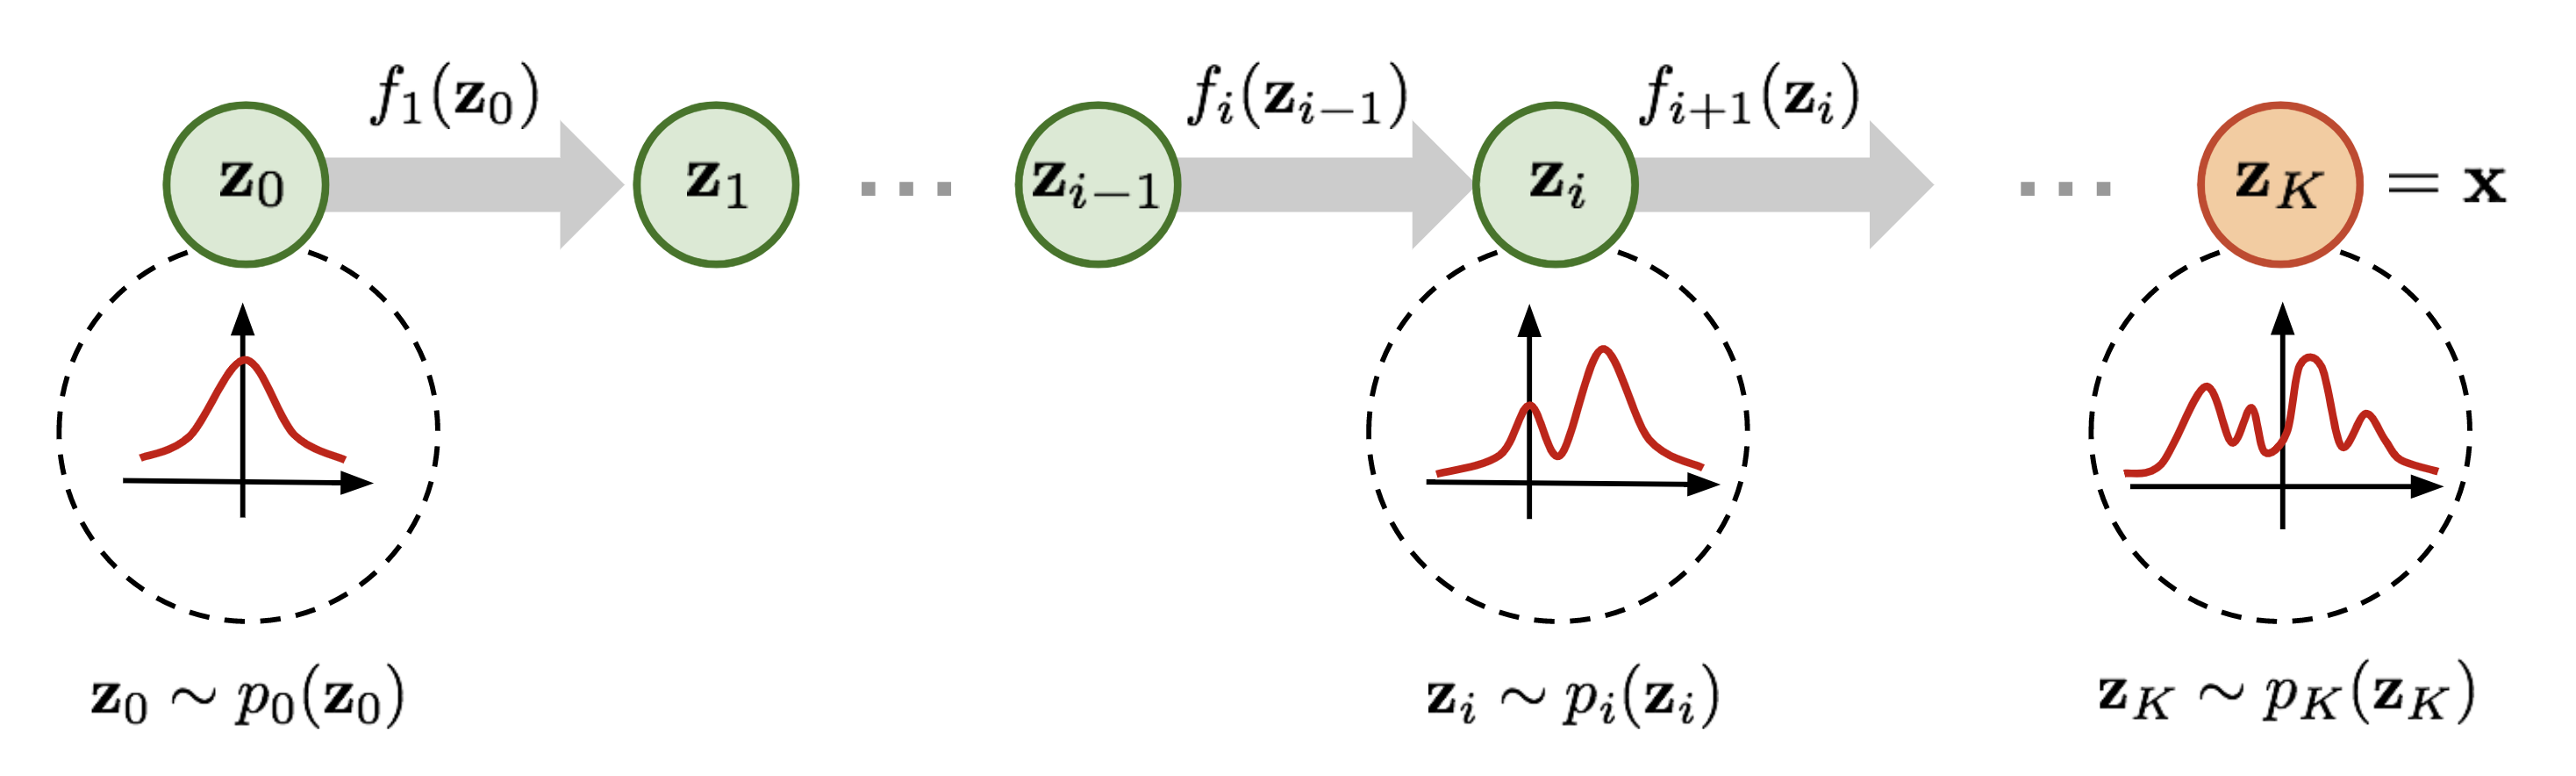
\includegraphics[width=0.95\linewidth]{figs/normalizing-flow}
	\end{figure}
	\vspace{-0.4cm}
	\[
		\log \pt(\bx) = \log p(\bff_K \circ \dots \circ \bff_1(\bx)) + \sum_{k=1}^K\log \left|\det \left(\frac{\partial \bff_k}{\partial \bff_{k-1}}\right)\right|.
	\]
	\vspace{-0.4cm}
\end{frame}
%=======
\begin{frame}{Towards Continuous-Time Normalizing Flows}
	\myfootnotewithlink{https://arxiv.org/abs/1906.02735}{Chen R. T. Q. et al. Residual Flows for Invertible Generative Modeling, 2019}
	Up to this point, we have considered discrete-time normalizing flows:
	\[
		\bx_{t+1} = \bff_{\btheta}(\bx_t, t); \quad \log p(\bx_{t+1}) = \log p(\bx_{t}) - \log \left| \det \frac{\partial \bff_{\btheta}(\bx_t)}{\partial \bx_{t}} \right| .
	\]
	\eqpause
	\begin{block}{Residual Flows}
		Let's condider the flow $\bff_{\btheta}(\bx, t) = \bx + \bv_{\btheta}(\bx, t)$:
		\[
			\bx_{t+1} = \bff_{\btheta}(\bx_t, t) = \bx_t + \bv_{\btheta}(\bx_t, t)
		\]
		\eqpause
		\vspace{-0.3cm}
		\begin{itemize}
			\item Here $\bff_{\btheta}$ is the NF \textbf{bijection}, $\bv_{\btheta}$ is the \textbf{velocity} (vector field).
			\item The update $\bx_{t+1} - \bx_t = \bv_{\btheta}(\bx_t, t)$ is a \textbf{finite-difference} approximation of a derivative.
		\end{itemize}
	\end{block}
\end{frame}
%=======
\begin{frame}{Towards Continuous-Time Normalizing Flows}
	Residual dynamics $\bx_{t+1} = \bx_t + \bv_{\btheta}(\bx_t, t)$ is an Euler step with $h=1$:
	\[
		\frac{\bx(t + h) - \bx(t)}{h} = \bv_{\btheta}(\bx(t), t)
	\]
	\eqpause
	Taking the limit $h \rightarrow 0$, we obtain continuous-time dynamics.
	\begin{block}{Continuous-Time Dynamics}
		Consider an Ordinary Differential Equation (ODE):
		\vspace{-0.3cm}
		\begin{align*}
		   \frac{d \bx(t)}{dt} &= \bv_{\btheta}(\bx(t), t); \quad \text{with initial condition }\bx(t_0) = \bx_0. \\
		   \nextonslide{
		   \bx(t_1) &= \int^{t_1}_{t_0} \bv_{\btheta}(\bx(t), t) d t  + \bx_0
		   }
		\end{align*}
		\vspace{-0.6cm}
	\end{block}
	Here, $\bv_{\btheta}: \bbR^m \times [t_0, t_1] \rightarrow \bbR^m$ is a \textbf{velocity vector field}.
\end{frame}
%=======
\begin{frame}{Ordinary Differential Equations (ODEs)}
	\begin{align*}
		\frac{d \bx(t)}{dt} &= \bv_{\btheta}(\bx(t), t); \quad \text{with initial condition }\bx(t_0) = \bx_0. \\
		\bx(t_1) &= \int^{t_1}_{t_0} \bv_{\btheta}(\bx(t), t) d t  + \bx_0
	\end{align*}
	\vspace{-0.6cm}
	\begin{block}{Flow}
		Let call \textbf{the flow} $\bpsi: \bbR^m \times [t_0, t_1] \rightarrow \bbR^m$ the solution of ODE:
		\[
			\frac{d \bpsi_t(\bx_0)}{dt} = \bv_{\btheta}(\bpsi_t(\bx_0), t); \quad \text{with initial condition }\bpsi_0(\bx_0) = \bx_0.
		\]
	\end{block}
	\begin{block}{Numerical Solution of ODEs}
		\vspace{-0.5cm}
		\[
			\bpsi_t(\bx_0) = \int^{t_1}_{t_0} \bv_{\btheta}(\bx(t), t) d t  + \bx_0 \nextonslide{\approx {\color{teal}\ODESolve_v(\bx_0, \btheta, t_0, t_1)}.}
		\]
		\eqpause
		Here, we require the numerical routine $\ODESolve_v(\bx_0, \btheta, t_0, t_1)$.
	\end{block}
\end{frame}
%=======
\begin{frame}{Numerical Solution of ODEs}
	\myfootnotewithlink{https://en.wikipedia.org/wiki/Heun's\_method}{Image credit: https://en.wikipedia.org/wiki/Heun's\_method}   
	\[
		\bpsi_t(\bx_0) = \int^{t_1}_{t_0} \bv_{\btheta}(\bx(t), t) d t  + \bx_0 \approx {\color{teal}\ODESolve_v(\bx_0, \btheta, t_0, t_1)}.
	\]
	$\ODESolve_v(\bx_0, \btheta, t_0, t_1)$ consists of sequence of iterative update steps.
	\eqpause
	\begin{block}{Euler Update Step}
		\begin{minipage}[t]{0.5\columnwidth}
			\vspace{-0.3cm}
			\[
	  			\frac{\bx(t + h) - \bx(t)}{h} = \bv_{\btheta}(\bx(t), t)
			\]
			\[
	  			\bx(t + h) = \bx(t) + h \cdot \bv_{\btheta}(\bx(t), t)
			\]
		\end{minipage}%
		\eqpause
		\begin{minipage}[t]{0.5\columnwidth}
			\vspace{-0.8cm}
			\begin{figure}
				\centering
				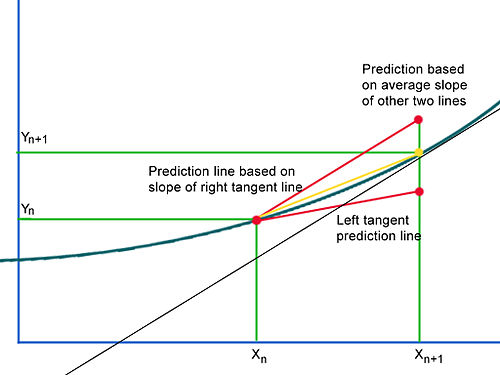
\includegraphics[width=\linewidth]{figs/heun_method}
			\end{figure}
		\end{minipage}
	\end{block}
	\vspace{-1.0cm}
	\begin{block}{Heun's Update Step}
		\vspace{-0.3cm}
		\[
			\bx'(t + h) = \bx(t) + h \cdot \bv_{\btheta}(\bx(t), t)
		\]
		\[
			\bx(t + h) = \bx(t) + \frac{h}{2} \cdot \left(\bv_{\btheta}(\bx(t), t) + \bv_{\btheta}(\bx'(t+h), t + h)\right)
		\]
	\end{block}
\end{frame}
%=======
\begin{frame}{Generative Models Taxonomy}
	\renderTaxonomy{ode}
\end{frame}
%=======
\begin{frame}{Continuous-Time Normalizing Flows: Neural ODE}
	\myfootnotewithlink{https://arxiv.org/abs/1806.07366}{Chen R. T. Q. et al. Neural Ordinary Differential Equations, 2018}   
	\begin{block}{Neural ODE}
		\vspace{-0.2cm}
		\[
  			\frac{d \bx(t)}{dt} = \bv_{\btheta}(\bx(t), t); \quad \text{with initial condition }\bx(t_0) = \bx_0
		\]
		\vspace{-0.3cm}
	\end{block}
	\begin{block}{Euler \ODESolve}
		\vspace{-0.3cm}
		\[
		    \bx(t + h) = \bx(t) + h \cdot \bv_{\btheta}(\bx(t), t)
		\]
		\vspace{-0.5cm}
	\end{block}
	\eqpause
	\begin{itemize}
		\item Consider $[t_0, t_1] = [0, 1]$ for simplicity.
		\item If $\bx(0)$ is a random variable with density~$p_0(\bx)$,
		\item Then, for any $t$, $\bx(t)$ is a random variable with density $p_t(\bx)$.
	\end{itemize}
\end{frame}
%=======
\begin{frame}{Continuous-Time Normalizing Flows: Intuition}
	\myfootnotewithlink{https://arxiv.org/abs/1810.01367}{Grathwohl W. et al. FFJORD: Free-form Continuous Dynamics for Scalable Reversible Generative Models, 2018}  
	\[
 		\frac{d \bx(t)}{dt} = \bv_{\btheta}(\bx(t), t); \quad \text{with initial condition }\bx(t_0) = \bx_0
	\]
	\eqpause
	\vspace{-0.5cm}
	\begin{itemize}
		\item $p_t(\bx) = p(\bx, t)$ describes the \textbf{probability path} interpolating between $p_0(\bx)$ and $p_1(\bx)$.
		\item {\color{gray}What is the difference between $p_t(\bx(t))$ and $p_t(\bx)$?}
	\end{itemize}
	\eqpause
	\begin{figure}
		\centering
		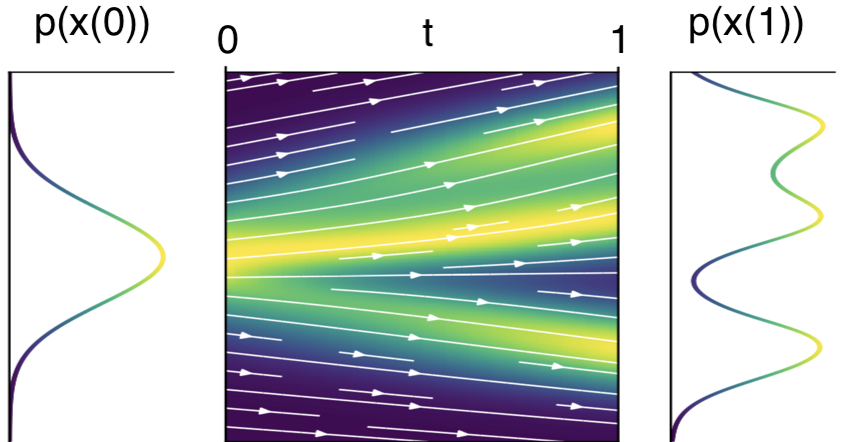
\includegraphics[width=0.75\linewidth]{figs/cnf_flow.png}
	\end{figure}
\end{frame}
%=======
\begin{frame}{Continuous-Time Normalizing Flows: Reversibility}
	\myfootnotewithlink{https://arxiv.org/abs/1806.07366}{Chen R. T. Q. et al. Neural Ordinary Differential Equations, 2018}   
	\begin{block}{Theorem (Picard)}
		If $\bv$ is continuously differentiable with a bounded derivative in $\bx$ and continuous in $t$, then the ODE has a \textbf{unique solution} given by a flow $\bpsi_t$.
	\end{block}
	\eqpause
	This guarantees the ODE is \textbf{uniquely reversible}. 
	\vspace{-0.3cm}
	\begin{align*}
		\bpsi_1(\bx_0) &= \bx_0 + \int_{0}^{1} \bv_{\btheta}(\bpsi_t(\bx_0), t) dt \\
		\bx(1) &= \bx(0) + \int_{0}^{1} \bv_{\btheta}(\bx(t), t) dt \\
		\bx(0) &= \bx(1) + \int_{1}^{0} \bv_{\btheta}(\bx(t), t) dt
	\end{align*}
	\eqpause
	\textbf{Note:} Unlike discrete-time flows, $\bv$ need not be invertible (uniqueness ensures bijection).
	\eqpause
	How can we compute $p_t(\bx)$ at arbitrary $t$?
\end{frame}
%=======
\begin{frame}{Summary}
	\begin{itemize}
		\item Continuous-time normalizing flows leverage neural ODEs to define continuous-time trajectories $\bx(t)$, relaxing many constraints of discrete-time flows.
		\vfill
		\item If $\bx_0$ is a random variable, this yields a \textbf{probability path} $p_t(\bx)$ as time evolves.
	\end{itemize}
\end{frame}
%=======
\end{document}